\begin{savequote}[75mm]
He who loves practice without theory is like the sailor who boards ship without a rudder and compass and never knows where he may cast.
\qauthor{Leonardo da Vinci}
\end{savequote}

\chapter{Self-Determination Theory}
\label{ChapterSDT}
Using key insights from my formative study (Chapter \ref{ChapterInteractNavi}), I designed and evaluated two equally important approaches, each focusing on a particular step in the driving navigation task. Towards my goal of rethinking route information and navigation guidance so that they can motivate drivers to choose unselfish routes, I sought to address two specific research questions. First, how can we encourage drivers to choose the unselfish route from a list of options before they even start a trip? Second, when they choose an unselfish option and start the trip, how do we make sure that they continue following that route? And if they choose otherwise, how can we convince them to switch to an available unselfish route along the way? From here on, I focus my attention to daily commutes because these trips are the main contributors to daily traffic, unlike trips to new locations which do not happen frequently. 

In this chapter, I discuss the characteristics of unselfish routes and how we can use Self-Determination Theory as as theoretical framework in designing future navigation applications as civic technology. 

\section{Unselfish Routes}

\begin{figure}[t]
  \centering
  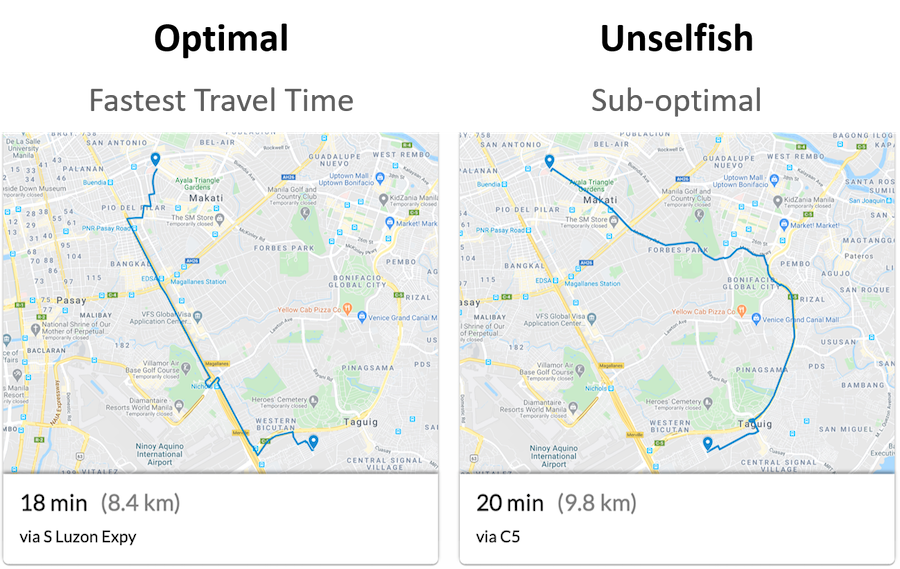
\includegraphics[scale=0.8]{figures/unselfish.png}
  \caption{Examples of an optimal and an unselfish route between home and work locations. }
  \label{fig:unselfish}
\end{figure}

Central to my dissertation is the recommendation of unselfish routes. In Wardrop's second principle (system optimal)\cite{wardrop1952road}, any route followed by a driver can be considered unselfish as long as it was chosen in cooperation with other drivers in the transportation network, and that these results to keeping the average journey time at a minimum. In Colak et. al.'s approach in modeling this problem, unselfish routes were characterized by the marginal cost they impose on other drivers in the same road segment\cite{colak2016understanding}. Whereas in Ringhand \& Volrath's investigation of factors that affect route choice, they characterized unselfish alternative routes as those with longer travel times or the route with more waits in traffic lights\cite{ringhand2018make}. 

For simplicity and consistency, here I define unselfish routes as alternative routes which have few overlaps with an optimal route in terms of roads included (Figure \ref{fig:unselfish}). They have longer distances and travel times, which make them sub-optimal for a driver. In practice, not all alternative routes should be recommended as unselfish. We still need to make sure that it is acceptable to the driver by ensuring its familiarity to the driver. Additionally, their time and distance differences are kept at a minimum, so that the unselfish route will not seem too novel. For these reasons, it can be a challenge to recommend them to drivers who already have regular routes to their everyday destinations. Further, choosing an unselfish route means drivers will have to give up or volunteer some of their time, which is not always ideal when going to or from work. 

\section{Navigation Apps as Civic Technology}

If future navigation applications will become tools to aid government stakeholders and urban planners in accomplishing their traffic management and sustainability goals, we have to start designing technical solutions from the point of view of civic technologies. By definition, civic technologies are tools that facilitate the collaboration between governments and their citizens for the public good\cite{Mandarano2010Civic}. In future traffic management systems, it would require a great amount of effort from governments to establish communication and technology platforms that will allow long term behavioral transformation among its citizens. On the part of the citizens, they have to be motivated enough in order to sustain or even be convinced that they should adopt or participate in such prosocial behavior. 

In our envisioned future, drivers on the road must collectively work together towards the common goal of avoiding traffic congestion. A more sustainable future is when citizens will voluntarily change their driving behaviors and daily routes because they are increasingly aware of its benefits for them and others.

Civic technologies have been used to organize citizens or small communities towards common goals. And in order for them to achieve tangible outcomes, citizens are usually asked to volunteer their time and effort for a number of reasons, most of the time without monetary incentives. Thus, despite effectively communicating lofty goals of achieving social good, designers of civic technologies still face the challenge of encouraging citizens to contribute and continue participation. In a similar context, it can be challenging to convince drivers that they should give up some of their time and choose an unselfish route for their daily commutes. 

Behavioral theories have been a cornerstone in HCI research especially in designing computing solutions that implement interventions for behavior change. The cross-pollination between the two fields have resulted to better interventions, systems and theories, and we have to continue this practice in order to achieve better behavioral outcomes \cite{hekler2013mind}. To inform my designs, I used Self-Determination Theory as a conceptual framework for the succeeding chapters.   

\section{Self-Determination Theory}
Motivation is the primary driving force in starting and performing any work, learning or task. These are often categorized as intrinsic and extrinsic motivation, wherein the former was proven to have positive effects on work performance\cite{gagne2005self}. One established theory on motivation, growth and well-being, the Self-Determination Theory (SDT)\cite{ryan2000intrinsic}, expands this categorization by introducing a spectrum of extrinsic motivation\cite{ryan2017self,deci2000and,deci2004handbook}. Past theories mainly consider the task as the origin of motivation. On the contrary, SDT posits that humans are active organisms that can regulate the internalization of external stimuli in developing one's self. We are given a framework to understand how humans who perform the task and their internalization of its reasons and goals affect their motivation\cite{ryan2013humans}. 

SDT is comprised of six mini-theories that characterizes different facets of motivation and personality functioning. Hereon, I will describe three mini-theories that primarily informed my designs. 

\subsection{Motivation}
SDT posits three types of motivation as shown in Figure \ref{fig:sdt}: intrinsic motivation, a spectrum of extrinsic motivation and amotivation. \textit{Intrinsic motivation} is the tendency of a person to pursue an activity or task because they find it inherently exciting, enjoyable or interesting, while \textit{extrinsic motivation} is the pursuit of an activity for an independent outcome (e.g. rewards, money). Devoid of any intention, a person who is \textit{amotivated} experience detachment from the task or activity that they are doing. But regardless of type, motivation always require energy to perform a task and this energy gets moved in a certain direction in the continuum\cite{deci2000and}(Figure \ref{fig:sdt}). Thus, when \textit{``an individual acquires an attitude, belief, or behavioral regulation and progressively transforms it into a personal value, goal, or organization,''}\cite{ryan2000intrinsic} these get internalized into autonomous and controlled motivation, or lack of motivation. As one person's motivation towards an activity moves to the right of the continuum, the motivational quality improves and the perceived locus of causality becomes internal, leading to stronger \textit{autonomous motivation}. But if the motivation's energy moves to the left of the continuum, the motivational quality of the activity becomes lower, requiring more \textit{controlled motivation} to perform a task. 

\begin{figure}[t]
  \centering
  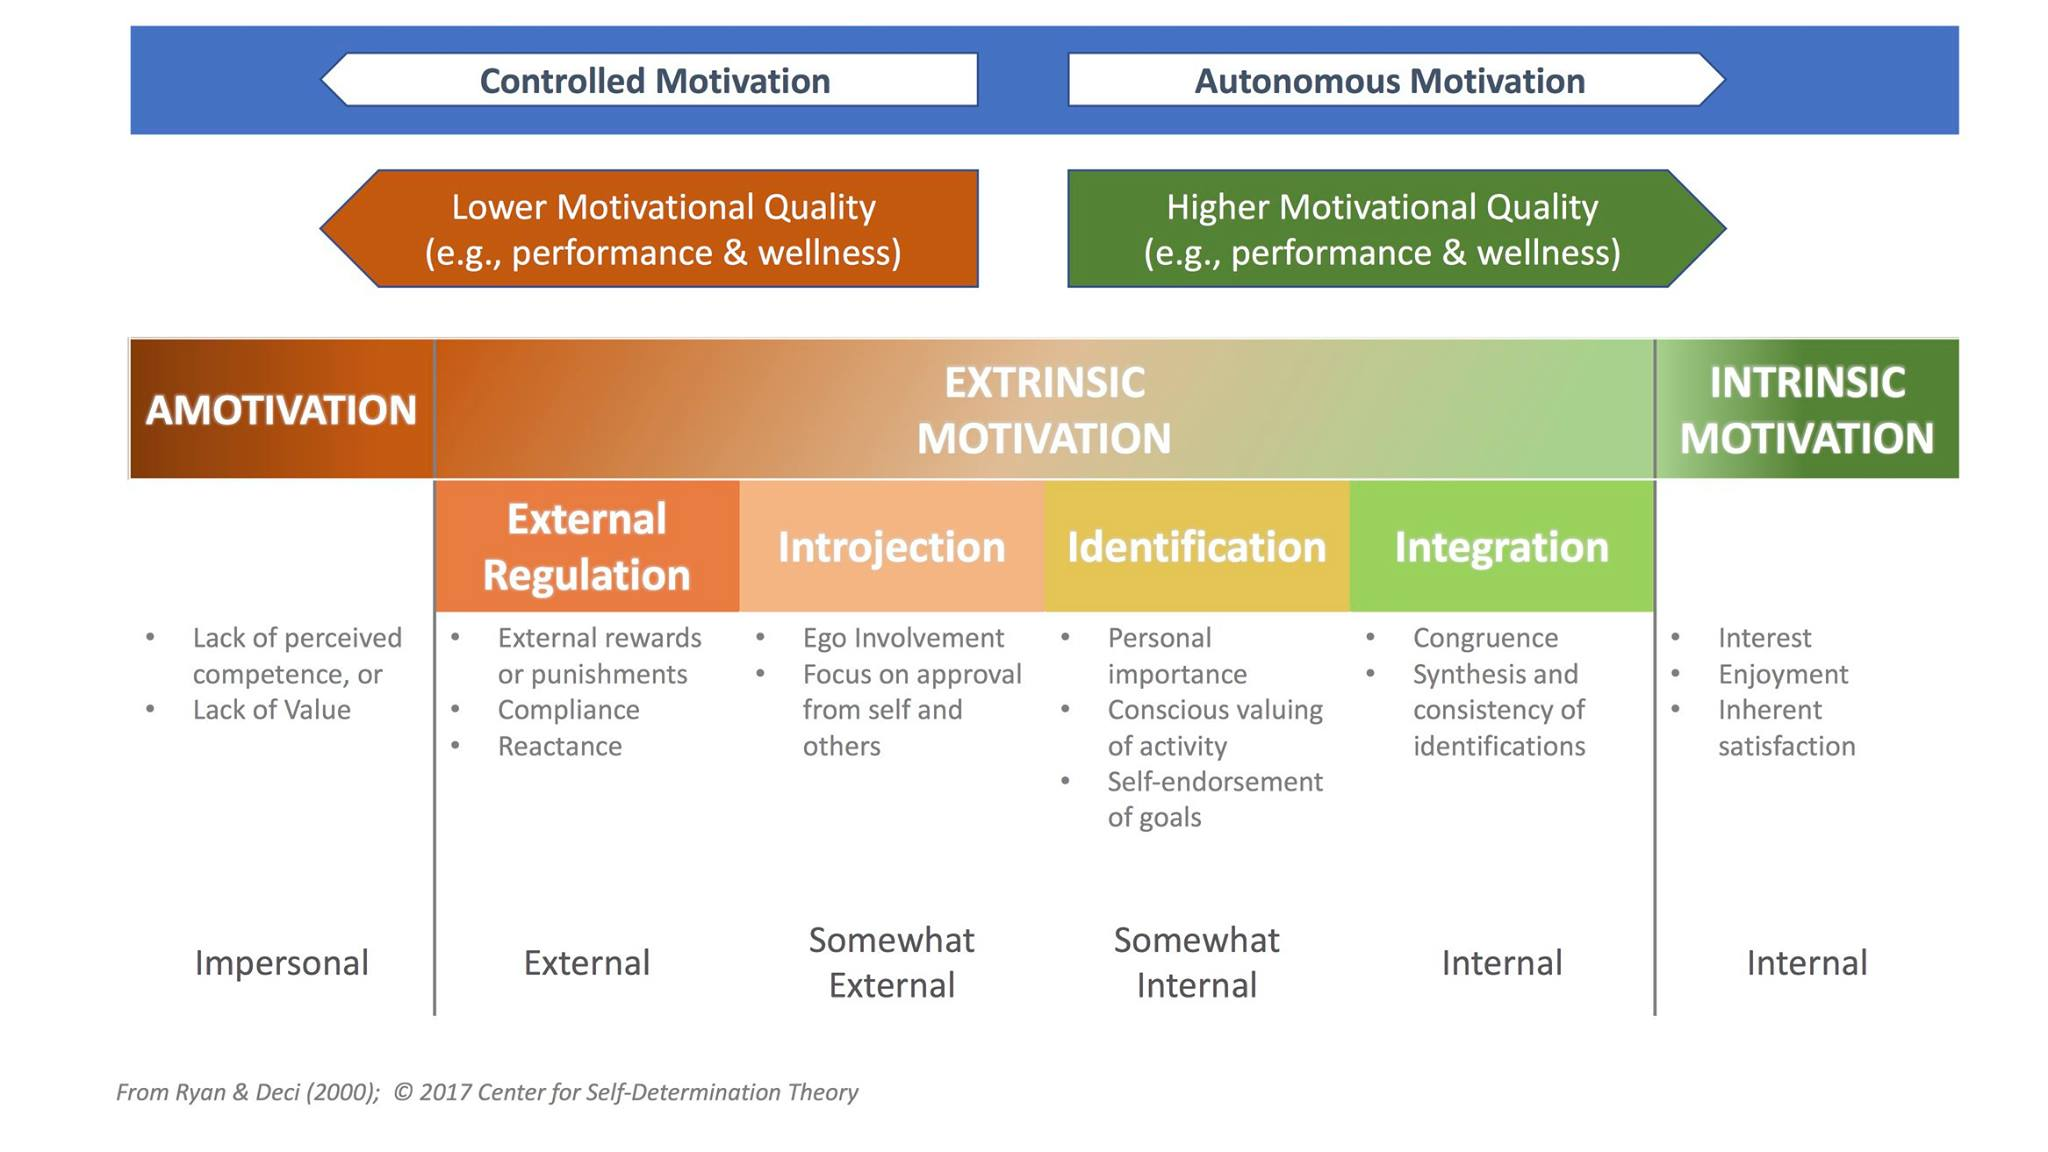
\includegraphics[scale=0.2]{figures/sdt.jpg}
  \caption{The different types of motivation and behavioral regulation. In this continuum, different forms of extrinsic motivation and behavioral regulation result to different motivational qualities. As you move to the right and develop a more self-determined extrinsic motivation, the motivational quality improves until intrinsic motivation is fostered. Going towards the left end of the spectrum means a person starts to lose whatever inherent interest they have and has to be controlled to perform a task with external rewards. This was adapted from \cite{ryan2000intrinsic,ryan2017organismic} and stylized by the Center for Self-Determination Theory.}
  \label{fig:sdt}
\end{figure}

There are two mini-theories that particularly address the facets of motivation. The first is \textit{Cognitive Evaluation Theory} (CET) which focuses on the factors that affect a person's \textit{intrinsic motivation} towards a task or activity. It states that social context and the functional significance of a stimulus or activity have an effect on need satisfaction and internalized intrinsic motivation\cite{deci2000and}. It emphasizes the importance of supporting the needs for competence and autonomy in developing \textit{intrinsic motivation} towards a task. However, it also posits that \textit{intrinsic motivation} can be diminished by the use of extrinsic rewards.  

The second mini-theory focuses on the various types of \textit{extrinsic motivation} and how they can be internalized by humans\cite{ryan2000intrinsic,deci2002overview,ryan2017organismic}. \textit{Organismic Integration Theory} (OIT) posits that \textit{extrinsic motivation} corresponds to behavior that aims for instrumental outcomes external from the activity itself. In a continuum (Figure \ref{fig:sdt}), the quality of extrinsic motivation changes based on how they are internally valued through internalization. In its least self-determined and internalized form, \textit{external regulation} is when a person acts purely for compliance or rewards. Moving towards the right of the continuum but still partially internalized, \textit{introjected regulation} is when someone acts out of guilt or for the approval of other people. It suggests that that person realizes the social value of the activity or task but has not fully aligned it yet with their personal values or goals. Moving towards an autonomous motivation, a person with \textit{identified regulation} performs a task or activity because they now see it as personally important. Lastly, the most self-determined form is when a person exhibits \textit{integrated regulation} or the performance of an activity because they perceive it as congruent to their personal values and goals, and are already internalized as part of their self. Thus, higher motivational quality can be achieved by working towards fully internalizing the extrinsic motivation. However, like in CET, the process of internalization is also affected by social contexts. And ensuring that the needs for autonomy and relatedness are supported can impact internalization. 

\subsection{General Causality Orientation}
In designing civic technologies, it is ideal that we engage citizens with causality orientations and behavioral regulation styles that foster autonomous motivation. SDT's framework describes a set of general causality orientations that describe ways people orient themselves across different environments and regulate their behavior. These temporally stable traits affect their perception of how self-determined their actions are. Persons who are autonomy oriented typically initiate tasks or activities on their own especially those that are interesting and challenging. They seek environments that are optimally challenging and allows choice. They take responsibility of their actions and when they encounter external events, they see it as informational rather than being controlled. Control oriented people usually act as a response to external demands like rewards, directives and ego involvements. They feel less autonomy because external events put pressure on them. Lastly, people with impersonal orientation tend to feel that they are not in control of situations and focus on obstacles towards intended outcomes. This makes them feel amotivated and leave things as they are. 

\subsection{Autonomous and Controlled Motivation}
If a person has a \textit{identification} or \textit{integration} regulatory style, and is autonomy oriented, they are predicted to internalize \textit{autonomous motivation}. On the other hand, if a person needs to be \textit{externally regulated} or has \textit{introjection} regulatory style, and is control oriented, they are predicted to internalize \textit{controlled motivation}. 

\subsection{Basic Psychological Needs}
In order to foster autonomous motivation and enhance the internalization of extrinsic motivation, SDT also claims that the environment within which a person performs a task must support three basic psychological needs that are universal: autonomy, competence and relatedness\cite{ryan2017basic}. Supporting the need for autonomy gives a sense that they are willingly performing self-endorsed actions. The need for competence requires us to make people feel they have an effect and to give them a sense of proficiency in their chosen work. Lastly, supporting the need for relatedness means providing a feeling of belonging and community with others. 

Thus, if we are to design future navigation applications as autonomy-supportive tools, the basic psychological needs have to be met, regardless of causality orientation and behavioral regulation style. To see how SDT can be implemented for navigation applications, the next chapter describes a GUI-based approach that adds motivative and familiarity information when displaying the list of choices to a driver.

% \begin{table}[h]
%     \caption{The general causality orientations according to the Self-Determination Theory framework.}
% 	\label{tab:gcos}
% 	\centering
% 	\begin{tabular}{l l}
% 	    \hline\hline
% 		\textbf{Autonomy orientation} & Oriented towards environments that stimulate intrinsic \\
%         & motivation, are optimally challenging, provide \\
%         & informational feedback, and allow choice. Tends to \\
%         & display greater self-initiation, seek activities that \\
%         & are interesting and challenging, and take greater responsibility \\
%         & for his or her own behavior. \\
%         & \\
%         \textbf{Controlled orientation} & Oriented toward being controlled by rewards, deadlines, \\
%         & structures, ego involvements, and the directives of others. \\
%         & Likely to be dependent on rewards or other controls, and may \\
%         & be more attuned to what others demand than to what they want \\
%         & for themselves \\
%         & \\
%         \textbf{Impersonal orientation} & Believes that attaining desired outcomes is beyond his or her \\
%         & control and that achievement is largely a matter of luck \\
%         & or fate. Likely to be anxious and feel very ineffective. \\
%         & Has no sense of being able to affect outcomes or cope \\ 
%         & with demands or changes. Tends to be amotivated and to want \\
%         & things to be as they always were. \\
% 		\hline
% 	\end{tabular}
% \end{table}